\section{Quy trình huấn luyện và các thực nghiệm chung}\label{sec:method}

Chương này trình bày pipeline huấn luyện, quy trình đánh giá và các kỹ thuật dùng chung cho cả bốn mô hình, sau đó báo cáo các thực nghiệm so sánh trên cùng một quy trình. Kết quả chi tiết của từng mô hình (siêu tham số cuối cùng, kết quả trên tập test, confusion matrix, feature importance) được trình bày riêng ở các Mục~\ref{sec:lr}--\ref{sec:xgb}.

\subsection{Kiến trúc tổng thể}
Mã nguồn được tổ chức thành các module độc lập trong thư mục \texttt{src/}, mỗi module đảm nhiệm một bước của pipeline:

\begin{table}[H]
\centering
\begin{adjustbox}{max width=\textwidth}
\begin{tabular}{|l|p{11.5cm}|}
\hline
\textbf{Module} & \textbf{Chức năng} \\
\hline
\texttt{data.py} & Đọc, kiểm tra và làm sạch dữ liệu; tải lại tập train/test theo danh sách \texttt{customerID} đã lưu. \\
\hline
\texttt{features.py} & Transformer \texttt{ChurnFeatureEngineer} tạo 9 đặc trưng mới (Experiment 2). \\
\hline
\texttt{preprocessing.py} & Xây dựng \texttt{ColumnTransformer} (imputation, One-Hot Encoding, scaling). \\
\hline
\texttt{models.py} & Khởi tạo bốn mô hình (có hoặc không có trọng số lớp) và quy định mô hình nào cần chuẩn hóa. \\
\hline
\texttt{train.py} & Chạy Stratified K-Fold Cross-Validation (\texttt{cv}) hoặc huấn luyện trên toàn bộ tập train và lưu pipeline (\texttt{fit}); tùy chọn \texttt{--feature-engineering} và \texttt{--imbalance}. \\
\hline
\texttt{compare.py} & So sánh hai lần chạy CV theo từng fold (paired): chênh lệch trung bình và số fold cải thiện. \\
\hline
\texttt{tune.py} & Tối ưu siêu tham số bằng \texttt{RandomizedSearchCV} trên đúng 5 fold, lưu pipeline tốt nhất. \\
\hline
\texttt{threshold.py} & Chọn ngưỡng quyết định trên xác suất out-of-fold của tập train (tối đa F1 hoặc F2). \\
\hline
\texttt{evaluate.py} & Nạp pipeline đã lưu và ngưỡng đã chọn, đánh giá trên tập test, vẽ Confusion Matrix, đường ROC và Precision--Recall. \\
\hline
\texttt{predict.py} & Dự đoán xác suất churn cho khách hàng mới từ file CSV. \\
\hline
\end{tabular}
\end{adjustbox}
\caption{Các module trong mã nguồn}
\end{table}

\begin{figure}[H]
\centering
\begin{tikzpicture}[
    node distance=0.6cm and 0.5cm,
    box/.style={rectangle, rounded corners, draw=black!70, fill=blue!8, minimum height=1cm, text width=2.3cm, align=center, font=\small},
    arrow/.style={-{Stealth[length=2.5mm]}, thick}
]
\node[box] (raw) {CSV gốc\\(7.043 dòng)};
\node[box, right=of raw] (clean) {Làm sạch\\\texttt{data.py}};
\node[box, right=of clean] (split) {Chia 80/20\\stratified};
\node[box, right=of split] (cv) {5-fold CV\\trên train};
\node[box, below=of cv] (fit) {Fit trên\\toàn bộ train};
\node[box, left=of fit] (test) {Đánh giá\\trên test};
\node[box, left=of test] (pred) {Dự đoán\\khách hàng mới};

\draw[arrow] (raw) -- (clean);
\draw[arrow] (clean) -- (split);
\draw[arrow] (split) -- (cv);
\draw[arrow] (cv) -- node[right, font=\footnotesize]{chọn cấu hình} (fit);
\draw[arrow] (fit) -- (test);
\draw[arrow] (test) -- (pred);
\end{tikzpicture}
\caption{Luồng xử lý của pipeline}
\end{figure}

Mỗi mô hình được đóng gói thành một \texttt{Pipeline} gồm các bước \texttt{features} (chỉ khi bật Feature Engineering), \texttt{preprocessor}, \texttt{smote} (chỉ khi dùng SMOTE) và \texttt{model}:

\begin{lstlisting}[style=pythonstyle, caption={Xây dựng pipeline huấn luyện trong \texttt{src/train.py} (rút gọn)}]
def build_training_pipeline(model_name, feature_engineering=False,
                            imbalance="none", balance_ratio=None):
    steps = []
    if feature_engineering:
        steps.append(("features", ChurnFeatureEngineer()))
    steps.append(("preprocessor", build_preprocessor(
        scale_numeric=requires_scaling(model_name),
        feature_engineering=feature_engineering)))
    if imbalance == "smote":
        steps.append(("smote", SMOTE(random_state=RANDOM_STATE)))
    steps.append(("model", build_model(
        model_name, random_state=RANDOM_STATE,
        balance_ratio=balance_ratio if imbalance == "class_weight" else None)))
    if imbalance == "smote":
        return ImbPipeline(steps=steps)  # chi resample khi fit
    return Pipeline(steps=steps)
\end{lstlisting}

Nhờ vậy, file \texttt{.joblib} được lưu chứa cả bộ tiền xử lý lẫn mô hình; \texttt{evaluate.py} và \texttt{predict.py} chỉ cần nạp lại file này mà không phải tiền xử lý thủ công. Mỗi lần chạy thực nghiệm đều lưu \texttt{config.json} (random state, số fold, danh sách đặc trưng, siêu tham số) cùng kết quả từng fold để có thể tái lập và đối chiếu.

\subsection{Cấu hình baseline của bốn mô hình}
Ở giai đoạn baseline, các mô hình dùng siêu tham số mặc định (hoặc gần mặc định), chưa tinh chỉnh và chưa xử lý mất cân bằng:

\begin{table}[H]
\centering
\begin{adjustbox}{max width=\textwidth}
\begin{tabular}{|l|p{9.5cm}|c|}
\hline
\textbf{Mô hình} & \textbf{Siêu tham số chính} & \textbf{Scaling} \\
\hline
Logistic Regression & \texttt{solver="lbfgs"}, \texttt{C=1.0}, \texttt{max\_iter=2000} & Có \\
\hline
Decision Tree & \texttt{criterion="gini"}, \texttt{max\_depth=None}, \texttt{min\_samples\_split=2} & Không \\
\hline
Random Forest & \texttt{n\_estimators=100}, \texttt{max\_features="sqrt"}, \texttt{max\_depth=None} & Không \\
\hline
XGBoost & \texttt{n\_estimators=100}, \texttt{learning\_rate=0.1}, \texttt{max\_depth=6}, \texttt{tree\_method="hist"} & Không \\
\hline
\end{tabular}
\end{adjustbox}
\caption{Cấu hình baseline (\texttt{random\_state=42} cho mọi mô hình)}
\end{table}

\subsection{Quy trình đánh giá}

\subsubsection{Cross-validation}
Việc so sánh và lựa chọn mô hình được thực hiện bằng \textbf{Stratified 5-Fold Cross-Validation} trên tập train (5.634 khách hàng). Các fold được sinh một lần với \texttt{random\_state=42} và dùng chung cho mọi mô hình, nên kết quả giữa các mô hình và giữa các lần chạy có thể so sánh trực tiếp. Kết quả được báo cáo dưới dạng \textit{trung bình $\pm$ độ lệch chuẩn} qua 5 fold; độ lệch chuẩn mô tả mức dao động giữa các fold, không phải khoảng tin cậy.

Ngoài điểm validation, nhóm ghi lại điểm trên phần huấn luyện của từng fold (\texttt{return\_train\_score=True}) để đo \textbf{khoảng cách train--validation}, dùng làm dấu hiệu nhận biết overfitting.

\subsubsection{Đánh giá cuối trên tập test}
Sau khi chọn cấu hình bằng cross-validation, quy trình cuối gồm ba lệnh:
\begin{enumerate}
    \item \texttt{python -m src.tune --fit}: tìm siêu tham số và lưu pipeline tốt nhất (đã huấn luyện lại trên toàn bộ tập train) vào \texttt{outputs/models/tuned/}.
    \item \texttt{python -m src.threshold}: chọn ngưỡng quyết định trên xác suất out-of-fold của tập train, ghi vào \texttt{thresholds.json}.
    \item \texttt{python -m src.evaluate --model-dir outputs/models/tuned}: đánh giá một lần duy nhất trên tập test 1.409 khách hàng với ngưỡng đã chọn.
\end{enumerate}
Mọi lựa chọn (cấu hình, siêu tham số, ngưỡng, mô hình cuối) đều được quyết định trước khi dùng tập test.

\subsubsection{Các chỉ số đánh giá}
Với lớp dương là ``rời bỏ'' (Churn $=1$), gọi TP, FP, TN, FN là các ô của Confusion Matrix:
\begin{align}
    \text{Accuracy}  &= \frac{TP + TN}{TP + TN + FP + FN} \\
    \text{Precision} &= \frac{TP}{TP + FP} \qquad
    \text{Recall} = \frac{TP}{TP + FN} \\
    \text{F1}        &= 2 \cdot \frac{\text{Precision} \cdot \text{Recall}}{\text{Precision} + \text{Recall}}
\end{align}
\begin{itemize}
    \item \textbf{Precision}: trong số khách hàng bị dự đoán rời bỏ, bao nhiêu phần trăm thực sự rời bỏ -- liên quan đến chi phí lãng phí ưu đãi.
    \item \textbf{Recall}: trong số khách hàng thực sự rời bỏ, mô hình phát hiện được bao nhiêu -- liên quan đến doanh thu bị mất do bỏ sót.
    \item \textbf{F1-score}: trung bình điều hòa của Precision và Recall, là chỉ số chính để so sánh trên dữ liệu mất cân bằng.
    \item \textbf{ROC-AUC}: diện tích dưới đường ROC, đo khả năng \textit{xếp hạng} khách hàng theo rủi ro, không phụ thuộc vào ngưỡng phân loại.
    \item \textbf{PR-AUC} (\textit{average precision}): diện tích dưới đường Precision--Recall. Cũng không phụ thuộc ngưỡng nhưng tập trung vào lớp thiểu số, nên nhạy hơn ROC-AUC khi dữ liệu mất cân bằng. Mức ngẫu nhiên của PR-AUC bằng tỉ lệ lớp dương (khoảng 0,265), trong khi của ROC-AUC là 0,5. PR-AUC là chỉ số dùng để chọn siêu tham số và mô hình cuối cùng.
\end{itemize}

\subsection{Các kỹ thuật cải thiện và giải thích mô hình}

\subsubsection{Xử lý mất cân bằng dữ liệu}
Lớp rời bỏ chỉ chiếm khoảng 26,5\% dữ liệu, nên ở ngưỡng mặc định 0,5 mô hình có xu hướng thiên về lớp đa số. Đề tài thử nghiệm ba cách xử lý:
\begin{itemize}
    \item \textbf{Class weight} (\textit{cost-sensitive learning}): gán trọng số lớn hơn cho lớp thiểu số trong hàm mất mát. Với trọng số ``balanced'', mẫu thuộc lớp $k$ có trọng số $w_k = \frac{n}{2\, n_k}$, khiến tổng trọng số của hai lớp bằng nhau. Với XGBoost, tương đương là \texttt{scale\_pos\_weight} $= n_{\text{neg}} / n_{\text{pos}} \approx 2{,}77$.
    \item \textbf{SMOTE} \cite{chawla2002}: sinh mẫu tổng hợp cho lớp thiểu số bằng nội suy giữa một mẫu $\mathbf{x}_i$ và một láng giềng gần nhất cùng lớp $\mathbf{x}_{nn}$: $\mathbf{x}_{\text{new}} = \mathbf{x}_i + \lambda(\mathbf{x}_{nn} - \mathbf{x}_i)$ với $\lambda \sim U(0, 1)$. SMOTE chỉ được áp dụng trên phần huấn luyện của mỗi fold.
    \item \textbf{Điều chỉnh ngưỡng quyết định}: thay vì dự đoán ``rời bỏ'' khi $\hat{p} > 0{,}5$, chọn ngưỡng $t$ tối đa một chỉ số mục tiêu (F1 hoặc F2) trên xác suất out-of-fold của tập train.
\end{itemize}

\subsubsection{Tối ưu siêu tham số}
\begin{itemize}
    \item \textbf{Grid Search:} thử toàn bộ tổ hợp trên lưới rời rạc; đơn giản nhưng chi phí tăng theo cấp số nhân với số siêu tham số.
    \item \textbf{Random Search} \cite{bergstra2012}: lấy mẫu ngẫu nhiên trong không gian tìm kiếm; với cùng ngân sách thường hiệu quả hơn Grid Search khi chỉ một số ít siêu tham số thực sự quan trọng. Đề tài sử dụng \texttt{RandomizedSearchCV} với các phân phối liên tục (ví dụ log-uniform cho \texttt{C} và \texttt{learning\_rate}).
    \item \textbf{Tối ưu Bayes / Optuna} \cite{akiba2019}: dùng kết quả các lần thử trước để đề xuất cấu hình tiếp theo; là hướng mở rộng khi không gian tìm kiếm lớn hơn.
\end{itemize}

\subsubsection{Giải thích mô hình}
\begin{itemize}
    \item \textbf{Hệ số Logistic Regression:} với đặc trưng đã chuẩn hóa, hệ số $\beta_j$ cho biết log-odds rời bỏ thay đổi bao nhiêu khi đặc trưng tăng một độ lệch chuẩn; tỉ số odds $e^{\beta_j}$ dễ diễn giải hơn.
    \item \textbf{Impurity importance} của mô hình cây: tổng mức giảm độ vẩn đục (Gini/entropy) tại các nút dùng đặc trưng đó, chuẩn hóa về tổng bằng 1. Cách tính nhanh nhưng thiên vị các đặc trưng liên tục có nhiều điểm chia.
    \item \textbf{Permutation importance} \cite{breiman2001}: xáo trộn ngẫu nhiên giá trị của một đặc trưng trên tập đánh giá và đo mức giảm của chỉ số (đề tài dùng PR-AUC). Cách này không phụ thuộc mô hình, làm việc trên 19 đặc trưng gốc nên dễ diễn giải, nhưng có thể đánh giá thấp các đặc trưng tương quan mạnh với nhau.
    \item \textbf{SHAP} \cite{lundberg2017} phân rã mỗi dự đoán thành tổng đóng góp của từng đặc trưng dựa trên giá trị Shapley, cho phép giải thích theo từng khách hàng; là hướng mở rộng của đề tài.
\end{itemize}

\subsection{Tổng quan các thực nghiệm}

Các thực nghiệm được thiết kế để trả lời từng câu hỏi riêng biệt. Mọi thực nghiệm dùng cùng tập train/test, cùng 5 fold Stratified và cùng tập chỉ số, chỉ thay đổi một yếu tố tại một thời điểm.

\begin{table}[H]
\centering
\begin{adjustbox}{max width=\textwidth}
\begin{tabular}{|c|p{6cm}|p{6.5cm}|}
\hline
\textbf{Thực nghiệm} & \textbf{Câu hỏi} & \textbf{Cách đánh giá} \\
\hline
1 & So sánh 4 thuật toán ở cấu hình baseline & 5-fold CV \\
\hline
2 & Feature Engineering có cải thiện hiệu năng? & 5-fold CV, so sánh cặp theo fold \\
\hline
3 & Class weight hay SMOTE giải quyết mất cân bằng tốt hơn? & 5-fold CV, so sánh cặp theo fold \\
\hline
4 & Hyperparameter Tuning cải thiện bao nhiêu? & RandomizedSearchCV trên cùng 5 fold \\
\hline
5 & Ngưỡng quyết định nào phù hợp? & Xác suất out-of-fold trên tập train \\
\hline
-- & Mô hình cuối cùng và giải thích mô hình & Tập test (dùng một lần) \\
\hline
\end{tabular}
\end{adjustbox}
\caption{Tổng quan các thực nghiệm}
\end{table}

So với kế hoạch ban đầu, nhóm không thực hiện thực nghiệm so sánh các phương pháp Encoding/Scaling; mọi thực nghiệm dùng chung One-Hot Encoding và \texttt{StandardScaler} (chỉ cho Logistic Regression).

% ============================================================
\subsection{Experiment 1: So sánh các mô hình baseline}\label{sec:exp1}
% ============================================================

\subsubsection{Kết quả cross-validation}

\begin{table}[H]
\centering
\small
\begin{adjustbox}{max width=\textwidth}
\begin{tabular}{|l|c|c|c|c|c|}
\hline
\textbf{Mô hình} & \textbf{Accuracy} & \textbf{Precision} & \textbf{Recall} & \textbf{F1} & \textbf{ROC-AUC} \\
\hline
Logistic Regression & \textbf{0,8019} $\pm$ 0,0133 & \textbf{0,6524} $\pm$ 0,0294 & \textbf{0,5431} $\pm$ 0,0460 & \textbf{0,5921} $\pm$ 0,0334 & \textbf{0,8461} $\pm$ 0,0140 \\
\hline
XGBoost             & 0,7982 $\pm$ 0,0088 & 0,6501 $\pm$ 0,0255 & 0,5204 $\pm$ 0,0235 & 0,5777 $\pm$ 0,0183 & 0,8413 $\pm$ 0,0084 \\
\hline
Random Forest       & 0,7863 $\pm$ 0,0092 & 0,6276 $\pm$ 0,0261 & 0,4803 $\pm$ 0,0215 & 0,5439 $\pm$ 0,0193 & 0,8199 $\pm$ 0,0114 \\
\hline
Decision Tree       & 0,7286 $\pm$ 0,0060 & 0,4890 $\pm$ 0,0108 & 0,4957 $\pm$ 0,0141 & 0,4922 $\pm$ 0,0082 & 0,6543 $\pm$ 0,0057 \\
\hline
\end{tabular}
\end{adjustbox}
\caption{Kết quả validation của 4 mô hình baseline (Stratified 5-fold CV trên tập train, 19 đặc trưng gốc)}
\label{tab:baseline_cv}
\end{table}

Nhận xét:
\begin{itemize}
    \item Theo F1 và ROC-AUC, thứ tự các mô hình là: \textbf{Logistic Regression $>$ XGBoost $>$ Random Forest $>$ Decision Tree}. Ở cấu hình mặc định, các mô hình dựa trên cây chưa vượt được mô hình tuyến tính.
    \item Logistic Regression và XGBoost rất gần nhau (chênh lệch F1 khoảng 0,014 và ROC-AUC khoảng 0,005, nhỏ hơn độ lệch chuẩn giữa các fold), nên chưa thể kết luận mô hình nào tốt hơn.
    \item Random Forest thấp hơn Logistic Regression khoảng 0,05 ở F1 và 0,026 ở ROC-AUC. Decision Tree thấp hơn hẳn, đặc biệt ROC-AUC chỉ 0,654 do cây không giới hạn độ sâu cho xác suất gần như chỉ nhận giá trị 0 hoặc 1.
    \item \textbf{Recall của cả bốn mô hình chỉ khoảng 0,48--0,54}: với ngưỡng mặc định 0,5, mô hình mới phát hiện được khoảng một nửa số khách hàng thực sự rời bỏ. Đây là điểm yếu chung cần cải thiện ở các thực nghiệm sau.
\end{itemize}

\subsubsection{Phân tích overfitting}

\begin{table}[H]
\centering
\begin{adjustbox}{max width=\textwidth}
\begin{tabular}{|l|c|c|c|c|c|c|}
\hline
\textbf{Mô hình} & \textbf{F1 train} & \textbf{F1 val} & \textbf{F1 gap} & \textbf{AUC train} & \textbf{AUC val} & \textbf{AUC gap} \\
\hline
Logistic Regression & 0,6018 & 0,5921 & 0,0096 & 0,8496 & 0,8461 & 0,0035 \\
\hline
XGBoost             & 0,7602 & 0,5777 & 0,1825 & 0,9504 & 0,8413 & 0,1091 \\
\hline
Random Forest       & 0,9968 & 0,5439 & 0,4529 & 0,9999 & 0,8199 & 0,1801 \\
\hline
Decision Tree       & 0,9968 & 0,4922 & 0,5046 & 1,0000 & 0,6543 & 0,3457 \\
\hline
\end{tabular}
\end{adjustbox}
\caption{Khoảng cách giữa điểm train và validation (trung bình 5 fold)}
\end{table}

\begin{itemize}
    \item \textbf{Logistic Regression} có điểm train và validation gần như trùng nhau: mô hình không overfit, nhưng điểm train thấp cho thấy mô hình tuyến tính có thể đang bị giới hạn về khả năng biểu diễn (\textit{underfit} nhẹ).
    \item \textbf{Decision Tree} và \textbf{Random Forest} gần như ghi nhớ hoàn toàn tập huấn luyện (F1 train $\approx 0{,}997$) do cây phát triển không giới hạn đến khi mỗi lá gần như thuần nhất. Random Forest giảm phương sai nhờ lấy trung bình nhiều cây (ROC-AUC validation tăng từ 0,654 lên 0,820) nhưng từng cây thành phần vẫn overfit.
    \item \textbf{XGBoost} cũng có dấu hiệu overfitting (F1 gap 0,18) ở cấu hình \texttt{max\_depth=6}, 100 cây.
    \item Kết luận: các mô hình cây có nhiều dư địa cải thiện nhất thông qua việc \textbf{giới hạn độ phức tạp} (\texttt{max\_depth}, \texttt{min\_samples\_leaf}, \texttt{min\_samples\_split}) và chính quy hóa -- là trọng tâm của Experiment 4.
\end{itemize}

\subsubsection{PR-AUC của các mô hình baseline}
Với dữ liệu mất cân bằng, nhóm ghi thêm PR-AUC cho mọi lần chạy. Ở cấu hình baseline, PR-AUC của Logistic Regression là 0,662, XGBoost 0,653, Random Forest 0,610 và Decision Tree chỉ 0,377 (mức ngẫu nhiên khoảng 0,265). Thứ hạng giống với F1 và ROC-AUC.

% ============================================================
\subsection{Experiment 2: Ảnh hưởng của Feature Engineering}
% ============================================================
\textbf{Thiết kế:} thêm bước \texttt{ChurnFeatureEngineer} (9 đặc trưng mới, Mục~\ref{sec:fe}) vào đầu pipeline, giữ nguyên mọi thứ khác (\texttt{python -m src.train cv --feature-engineering}). Để kiểm tra FE có giúp ích khi đã xử lý mất cân bằng hay không, nhóm chạy FE trong cả ba bối cảnh: không xử lý, class weight và SMOTE. Mỗi so sánh được thực hiện \textbf{theo cặp trên từng fold} (\texttt{src/compare.py}): vì mọi lần chạy dùng cùng 5 fold, chênh lệch được tính trên từng fold rồi lấy trung bình, kèm số fold mà cấu hình có FE tốt hơn.

\begin{table}[H]
\centering
\small
\begin{adjustbox}{max width=\textwidth}
\begin{tabular}{|l|c|c|c|c|c|c|}
\hline
\multirow{2}{*}{\textbf{Mô hình}} & \multicolumn{2}{c|}{\textbf{Không xử lý}} & \multicolumn{2}{c|}{\textbf{Class weight}} & \multicolumn{2}{c|}{\textbf{SMOTE}} \\
\cline{2-3} \cline{4-5} \cline{6-7}
 & $\Delta$F1 & $\Delta$PR-AUC & $\Delta$F1 & $\Delta$PR-AUC & $\Delta$F1 & $\Delta$PR-AUC \\
\hline
Logistic Regression & +0,003 (3/5) & +0,001 (3/5) & +0,001 (2/5) & +0,001 (3/5) & +0,000 (2/5) & $-$0,000 (2/5) \\
\hline
Decision Tree & +0,003 (3/5) & +0,003 (3/5) & $-$0,009 (1/5) & $-$0,008 (2/5) & +0,005 (3/5) & +0,003 (3/5) \\
\hline
Random Forest & $-$0,010 (2/5) & +0,008 (3/5) & $-$0,005 (1/5) & +0,007 (4/5) & +0,010 (3/5) & +0,007 (4/5) \\
\hline
XGBoost & $-$0,012 (1/5) & $-$0,007 (1/5) & $-$0,004 (3/5) & $-$0,003 (3/5) & $-$0,010 (1/5) & $-$0,006 (1/5) \\
\hline
\end{tabular}
\end{adjustbox}
\caption{Chênh lệch khi thêm Feature Engineering (trung bình 5 fold; trong ngoặc: số fold cải thiện)}
\label{tab:fe}
\end{table}

\subsubsection{Phân tích}
\begin{itemize}
    \item \textbf{Feature Engineering không mang lại cải thiện đáng kể.} Mọi chênh lệch đều nằm trong khoảng $\pm 0{,}012$, nhỏ hơn độ lệch chuẩn của F1 giữa các fold (0,02--0,03), và không có cấu hình nào cải thiện ở cả 5 fold. Kết quả nhất quán trong cả ba bối cảnh xử lý mất cân bằng.
    \item \textbf{XGBoost giảm nhẹ trong cả ba bối cảnh} (F1 giảm 0,004--0,012, chỉ cải thiện ở 1--3/5 fold). Ở cấu hình mặc định (\texttt{max\_depth=6}), XGBoost đã overfit (Mục~\ref{sec:exp1}); thêm các đặc trưng liên tục như \texttt{avg\_monthly\_charge}, \texttt{charge\_diff} tạo thêm điểm chia để mô hình khớp nhiễu. F1 train của XGBoost tăng từ 0,760 lên 0,790 trong khi F1 validation giảm.
    \item \textbf{Random Forest tăng nhẹ PR-AUC} (+0,007 đến +0,008, cải thiện ở 3--4/5 fold) nhưng F1 lúc tăng lúc giảm, nên không đủ cơ sở kết luận.
    \item \textbf{Nguyên nhân:} các đặc trưng mới đều được dựng từ thông tin mô hình đã có. Mô hình cây tự học được các ngưỡng (ví dụ \texttt{tenure} $\le 12$) và tương tác (hợp đồng $\times$ thời gian sử dụng), còn Logistic Regression đã nắm được xu hướng chính qua \texttt{tenure}, \texttt{Contract} và \texttt{InternetService}.
    \item \textbf{Kết luận:} FE không được đưa vào cấu hình cuối cùng; các thực nghiệm sau dùng 19 đặc trưng gốc.
\end{itemize}

% ============================================================
\subsection{Experiment 3: Xử lý mất cân bằng dữ liệu}\label{sec:exp3}
% ============================================================
\textbf{Thiết kế:} giữ nguyên 19 đặc trưng gốc và siêu tham số baseline, chỉ thay đổi cách xử lý mất cân bằng (\texttt{--imbalance}):
\begin{itemize}
    \item \textbf{Class weight:} \texttt{class\_weight="balanced"} cho Logistic Regression, Decision Tree, Random Forest; với XGBoost dùng \texttt{scale\_pos\_weight} bằng tỉ lệ số mẫu không rời bỏ / rời bỏ ($4.139 / 1.495 \approx 2{,}77$). Cả hai cách đều làm tổng trọng số của hai lớp bằng nhau.
    \item \textbf{SMOTE:} chèn bước \texttt{SMOTE} sau \texttt{preprocessor} trong \texttt{imblearn.pipeline.}\allowbreak\texttt{Pipeline}. Pipeline của \texttt{imblearn} chỉ sinh mẫu khi \texttt{fit}, nên SMOTE chỉ tác động lên phần huấn luyện của mỗi fold; fold validation và tập test giữ nguyên phân bố thật.
\end{itemize}

\begin{table}[H]
\centering
\small
\begin{adjustbox}{max width=\textwidth}
\begin{tabular}{|l|l|c|c|c|c|c|}
\hline
\textbf{Mô hình} & \textbf{Chiến lược} & \textbf{Precision} & \textbf{Recall} & \textbf{F1} & \textbf{$\Delta$F1 (fold)} & \textbf{PR-AUC} \\
\hline
\multirow{3}{*}{Logistic Regression} & Không xử lý & 0,652 & 0,543 & 0,592 & -- & 0,662 \\
\cline{2-7}
 & Class weight & 0,517 & \textbf{0,801} & 0,628 & +0,036 (5/5) & 0,660 \\
\cline{2-7}
 & SMOTE & 0,526 & 0,789 & \textbf{0,631} & +0,039 (5/5) & 0,658 \\
\hline
\multirow{3}{*}{Decision Tree} & Không xử lý & 0,489 & 0,496 & 0,492 & -- & 0,377 \\
\cline{2-7}
 & Class weight & 0,512 & 0,496 & \textbf{0,504} & +0,012 (4/5) & 0,389 \\
\cline{2-7}
 & SMOTE & 0,479 & 0,495 & 0,487 & $-$0,006 (1/5) & 0,372 \\
\hline
\multirow{3}{*}{Random Forest} & Không xử lý & 0,628 & 0,480 & 0,544 & -- & 0,610 \\
\cline{2-7}
 & Class weight & 0,563 & \textbf{0,638} & \textbf{0,598} & +0,054 (5/5) & 0,604 \\
\cline{2-7}
 & SMOTE & 0,608 & 0,496 & 0,546 & +0,002 (3/5) & 0,593 \\
\hline
\multirow{3}{*}{XGBoost} & Không xử lý & 0,650 & 0,520 & 0,578 & -- & 0,653 \\
\cline{2-7}
 & Class weight & 0,545 & \textbf{0,747} & \textbf{0,630} & +0,053 (5/5) & 0,653 \\
\cline{2-7}
 & SMOTE & 0,636 & 0,565 & 0,598 & +0,020 (5/5) & 0,651 \\
\hline
\end{tabular}
\end{adjustbox}
\caption{Kết quả validation (5-fold CV, ngưỡng 0,5) của các chiến lược xử lý mất cân bằng}
\label{tab:imbalance}
\end{table}

\subsubsection{Phân tích}
\begin{itemize}
    \item \textbf{Class weight là chiến lược tốt và ổn định nhất.} F1 tăng 0,036--0,054 và tăng ở cả 5/5 fold với Logistic Regression, Random Forest và XGBoost. Recall tăng mạnh: Logistic Regression từ 0,543 lên 0,801, XGBoost từ 0,520 lên 0,747. Mô hình giờ phát hiện được khoảng 3/4 khách hàng rời bỏ thay vì một nửa.
    \item \textbf{Cái giá là Precision giảm} (Logistic Regression: 0,652 xuống 0,517; XGBoost: 0,650 xuống 0,545): mô hình chấp nhận cảnh báo nhầm nhiều hơn để bắt được nhiều khách hàng rời bỏ hơn. Vì Recall tăng nhiều hơn Precision giảm, F1 vẫn tăng. Với bài toán giữ chân khách hàng, bỏ sót một khách hàng sắp rời bỏ thường tốn kém hơn gửi nhầm một ưu đãi, nên đánh đổi này là hợp lý.
    \item \textbf{PR-AUC gần như không đổi} ($|\Delta| \le 0{,}006$ với LR, RF, XGBoost). Class weight không làm mô hình \textit{xếp hạng} khách hàng tốt hơn mà chủ yếu \textit{dịch chuyển xác suất dự đoán} lên cao, tương đương với hạ ngưỡng quyết định.
    \item \textbf{SMOTE hiệu quả với Logistic Regression} (+0,039 F1, tương đương class weight) nhưng yếu hơn với mô hình cây: XGBoost chỉ +0,020, Random Forest gần như không đổi. SMOTE nội suy tuyến tính giữa các mẫu sau One-Hot Encoding nên tạo ra các giá trị không có thật (ví dụ 0,4 cho cột \texttt{Contract\_Two year}); mô hình cây chia theo ngưỡng nên dễ bị ảnh hưởng bởi các mẫu giả này. Class weight đơn giản hơn và không sinh dữ liệu giả.
    \item \textbf{Decision Tree gần như không phản ứng} (Recall vẫn 0,496), và Recall của Random Forest chỉ tăng lên 0,638. Ở cấu hình mặc định, cây phát triển đến khi lá thuần nhất (F1 train $\approx 0{,}997$), nên xác suất dự đoán gần như chỉ là 0 hoặc 1; trọng số lớp không còn tác dụng khi mọi lá đã thuần nhất. Điều này chỉ thay đổi sau khi giới hạn độ phức tạp ở Experiment 4.
    \item \textbf{Kết luận:} chọn \textbf{class weight} cho mọi mô hình ở các bước tiếp theo.
\end{itemize}

% ============================================================
\subsection{Experiment 4: Hyperparameter Tuning}\label{sec:exp4}
% ============================================================
\textbf{Thiết kế:} tối ưu siêu tham số bằng \texttt{RandomizedSearchCV} (\texttt{python -m src.tune}) trên cấu hình class weight, 19 đặc trưng gốc. Tìm kiếm dùng đúng 5 fold của các thực nghiệm trước, nên kết quả so sánh cặp được với Experiment 3. Tiêu chí chọn là \textbf{PR-AUC} vì chỉ số này không phụ thuộc ngưỡng và tập trung vào lớp rời bỏ; ngưỡng được chọn riêng ở Experiment 5.

\begin{table}[H]
\centering
\small
\begin{adjustbox}{max width=\textwidth}
\begin{tabular}{|l|c|p{9.8cm}|}
\hline
\textbf{Mô hình} & \textbf{Số tổ hợp} & \textbf{Không gian tìm kiếm} \\
\hline
Logistic Regression & 30 & \texttt{C} $\sim$ log-uniform$(10^{-3}, 10^{2})$ \\
\hline
Decision Tree & 50 & \texttt{max\_depth} $\in [2, 15]$, \texttt{min\_samples\_leaf} $\in [1, 59]$, \texttt{criterion} $\in$ \{gini, entropy\} \\
\hline
Random Forest & 40 & \texttt{n\_estimators} $\in [200, 600]$, \texttt{max\_depth} $\in$ \{4, 6, 8, 10, 12, 16, None\}, \texttt{min\_samples\_leaf} $\in [1, 29]$, \texttt{max\_features} $\in$ \{sqrt, log2, 0,5\} \\
\hline
XGBoost & 60 & \texttt{n\_estimators} $\in [100, 600]$, \texttt{learning\_rate} $\sim$ log-uniform$(0{,}01; 0{,}3)$, \texttt{max\_depth} $\in [2, 7]$, \texttt{min\_child\_weight} $\in [1, 10]$, \texttt{subsample}, \texttt{colsample\_bytree} $\in [0{,}6; 1]$, \texttt{reg\_lambda} $\sim$ log-uniform$(0{,}1; 10)$ \\
\hline
\end{tabular}
\end{adjustbox}
\caption{Không gian tìm kiếm siêu tham số}
\end{table}

Siêu tham số tốt nhất của từng mô hình được trình bày ở các Mục~\ref{sec:lr}--\ref{sec:xgb}.

\subsubsection{Kết quả}

\begin{table}[H]
\centering
\small
\begin{adjustbox}{max width=\textwidth}
\begin{tabular}{|l|c|c|c|c|c|c|}
\hline
\textbf{Mô hình} & \textbf{Recall} & \textbf{F1} & \textbf{$\Delta$F1 (fold)} & \textbf{ROC-AUC} & \textbf{PR-AUC} & \textbf{$\Delta$PR-AUC (fold)} \\
\hline
Logistic Regression & 0,801 & 0,628 & +0,000 (2/5) & 0,846 & 0,660 & +0,000 (5/5) \\
\hline
Decision Tree & 0,799 & 0,621 & \textbf{+0,117 (5/5)} & 0,830 & 0,630 & \textbf{+0,242 (5/5)} \\
\hline
Random Forest & 0,776 & 0,631 & +0,033 (5/5) & 0,848 & 0,667 & +0,063 (5/5) \\
\hline
XGBoost & \textbf{0,806} & \textbf{0,632} & +0,002 (3/5) & \textbf{0,850} & \textbf{0,671} & +0,018 (5/5) \\
\hline
\end{tabular}
\end{adjustbox}
\caption{Kết quả validation sau tuning (class weight, ngưỡng 0,5). Chênh lệch so với class weight với siêu tham số mặc định (Experiment 3).}
\label{tab:tuning}
\end{table}

\subsubsection{Phân tích}
\begin{itemize}
    \item \textbf{Tuning giải quyết được overfitting của mô hình cây.} Khoảng cách F1 train--validation giảm từ 0,49 xuống 0,03 với Decision Tree, từ 0,39 xuống 0,07 với Random Forest và từ 0,16 xuống 0,03 với XGBoost. Các cấu hình được chọn đều đơn giản hơn mặc định: lá có ít nhất 11--51 mẫu, cây sâu tối đa 3--12, XGBoost dùng learning rate nhỏ (0,023).
    \item \textbf{Decision Tree hưởng lợi nhiều nhất}: PR-AUC tăng từ 0,389 lên 0,630, ROC-AUC từ 0,663 lên 0,830, cải thiện ở cả 5 fold. Random Forest tăng 0,063 PR-AUC. XGBoost tăng ít hơn (+0,018 PR-AUC) vì mặc định đã có một số cơ chế chống overfit (learning rate, chính quy hóa), nhưng vẫn cải thiện ở cả 5 fold.
    \item \textbf{Class weight giờ mới phát huy tác dụng với mô hình cây.} Recall của Decision Tree tăng từ 0,496 lên 0,799 và Random Forest từ 0,638 lên 0,776. Khi lá không còn thuần nhất, xác suất dự đoán mịn hơn và trọng số lớp mới thực sự dịch chuyển được quyết định -- giải thích vì sao ở Experiment 3, class weight gần như không tác động lên Decision Tree.
    \item \textbf{Logistic Regression không đổi} (\texttt{C=0,92} gần mặc định 1,0): mô hình vốn không overfit (khoảng cách train--validation 0,01), giới hạn của nó nằm ở dạng tuyến tính chứ không ở siêu tham số.
    \item \textbf{Sau tuning, bốn mô hình rất sát nhau} (F1 0,621--0,632, PR-AUC 0,630--0,671). XGBoost có PR-AUC và ROC-AUC cao nhất nhưng chênh lệch với Random Forest (0,004 PR-AUC) nhỏ hơn độ lệch chuẩn giữa các fold (0,02).
    \item \textbf{Lưu ý:} siêu tham số được chọn và chấm điểm trên cùng 5 fold, nên điểm sau tuning hơi lạc quan. Kết quả trên tập test (Mục~\ref{sec:final_test}) cho thấy mức lạc quan này nhỏ.
\end{itemize}

% ============================================================
\subsection{Experiment 5: Chọn ngưỡng quyết định}\label{sec:exp5}
% ============================================================
\textbf{Thiết kế:} với mỗi pipeline đã tuning, \texttt{src/threshold.py} chạy lại 5-fold CV trên tập train để lấy \textbf{xác suất out-of-fold}: mỗi khách hàng được dự đoán bởi mô hình không thấy khách hàng đó lúc huấn luyện. Ngưỡng được quét từ 0,05 đến 0,95 (bước 0,01) và chọn theo hai tiêu chí: tối đa F1 (ngưỡng chính) và tối đa F2 (coi Recall quan trọng gấp đôi Precision). Tập test không tham gia vào bước này.

\begin{table}[H]
\centering
\small
\begin{adjustbox}{max width=\textwidth}
\begin{tabular}{|l|c|c|c|c|c|c|}
\hline
\textbf{Mô hình} & \textbf{Ngưỡng F1} & \textbf{F1 ở 0,5} & \textbf{F1 ở ngưỡng F1} & \textbf{Fold cải thiện} & \textbf{Ngưỡng F2} & \textbf{Recall ở ngưỡng F2} \\
\hline
Logistic Regression & 0,60 & 0,629 & 0,637 & 4/5 & 0,32 & 0,922 \\
\hline
Decision Tree & 0,60 & 0,620 & 0,628 & 3/5 & 0,26 & 0,910 \\
\hline
Random Forest & 0,60 & 0,631 & 0,639 & 4/5 & 0,34 & 0,889 \\
\hline
XGBoost & 0,57 & 0,632 & 0,639 & 3/5 & 0,37 & 0,887 \\
\hline
\end{tabular}
\end{adjustbox}
\caption{Ngưỡng được chọn trên xác suất out-of-fold của tập train}
\label{tab:threshold}
\end{table}

\begin{figure}[H]
\centering
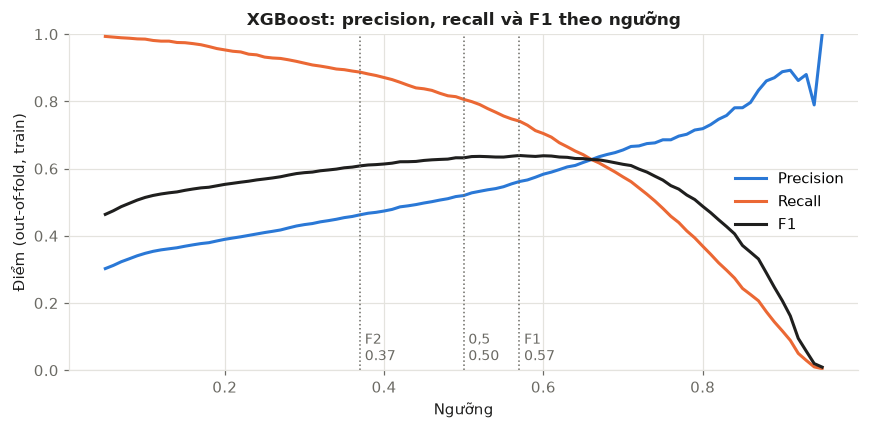
\includegraphics[width=0.7\textwidth]{img/nb_threshold_xgb.png}
\caption{Precision, Recall và F1 của XGBoost theo ngưỡng (out-of-fold trên tập train)}
\label{fig:threshold}
\end{figure}

\subsubsection{Phân tích}
\begin{itemize}
    \item \textbf{Ngưỡng tối ưu F1 cao hơn 0,5} (0,57--0,60). Class weight đã đẩy xác suất dự đoán lên cao, khiến ở ngưỡng 0,5 mô hình nghiêng hẳn về Recall (khoảng 0,80); ngưỡng tối ưu F1 kéo cân bằng ngược lại một chút về phía Precision.
    \item \textbf{Mức cải thiện F1 nhỏ} (+0,007 đến +0,008) và chỉ ở 3--4/5 fold. Đường F1 khá phẳng trong khoảng 0,45--0,65 (Hình~\ref{fig:threshold}), nên chọn ngưỡng nào trong khoảng này cũng cho F1 gần như nhau. Vai trò chính của ngưỡng là \textit{điều chỉnh cân bằng Precision--Recall} theo nhu cầu kinh doanh, không phải tăng F1.
    \item \textbf{Ngưỡng F2} (0,26--0,37) cho Recall 0,89--0,92 nhưng F1 giảm 0,02--0,05: phù hợp khi doanh nghiệp coi việc bỏ sót khách hàng rời bỏ tốn kém hơn nhiều so với gửi nhầm ưu đãi.
\end{itemize}
